\part{Discrétisation et Implémentation}
\label{partImp}

Une fois les différents problèmes correctement posés, il s'agit d'implémenter un code pour les résoudre. Ceci est fait avec la bibliothèque Feel++, qui permet de manipuler en C++ des objets permettant la résolution d'équations aux dérivées partielles par des méthodes de Galerkin continues et discontinues (voir \ref{eltfinis}). Ces objets peuvent correspondre au maillage, aux formes variationnelles ainsi que plusieurs solveurs linéaires et pré-conditionneurs grâce à PETSc \cite{petsc-web-page,petsc-user-ref,petsc-efficient} et des solveurs de problèmes aux valeurs propres grâce à SLEPc \cite{Hernandez:2005:SSF}.\\

D'abord, il faut choisir une géométrie sur laquelle travaillé. On prend donc un cylindre de diamètre 1 et de longueur 5, orienté dans l'axe $z$. La géométrie est notée $\Omega$ et le bord de la géométrie est noté $\Gamma$ ou $\partial\Omega$. $\Gamma$ se décompose en trois partie, l'entrée $\Gamma_1$,  la sortie $\Gamma_2$ et le tour noté $\Gamma_3$, comme montré dans la figure \ref{figMesh}, sa conception est détaillé dans l'annexe \ref{mesh}.\\
\begin{figure}[H]
\centering
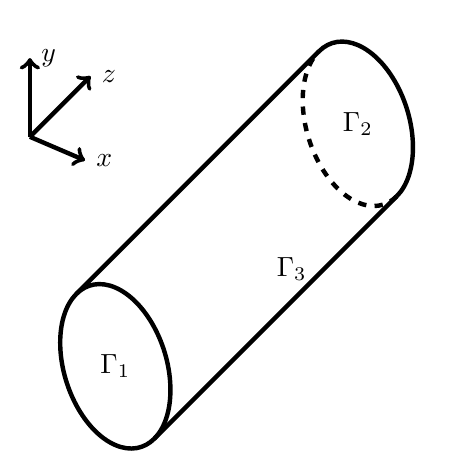
\begin{tikzpicture}
\begin{scope}[x={(.7cm,-.3cm)}]
\path (1,0,0);
\pgfgetlastxy{\cylxx}{\cylxy}
\path (0,1,0);
\pgfgetlastxy{\cylyx}{\cylyy}
\path (0,0,1);
\pgfgetlastxy{\cylzx}{\cylzy}
\pgfmathsetmacro{\cylt}{(\cylzy * \cylyx - \cylzx * \cylyy)/ (\cylzy * \cylxx - \cylzx * \cylxy)}
\pgfmathsetmacro{\ang}{atan(\cylt)}
\pgfmathsetmacro{\ct}{1/sqrt(1 + (\cylt)^2)}
\pgfmathsetmacro{\st}{\cylt * \ct}
\begin{scope}[every path/.style={ultra thick}]
\draw (0,0,0) circle[radius=1];
\draw[->] (-1,3,1) -- (0,3,1);
\draw (0,3,1) node [right] {$x$};
\draw[->] (-1,3,1) -- (-1,4,1);
\draw (-1,4,1) node [right] {$y$};
\draw[->] (-1,3,1) -- (-1,3,-1);
\draw (-1,3,-1) node [right] {$z$};
\draw (\ct,\st,0) -- ++(0,0,-8);
\draw (-\ct,-\st,0) -- ++(0,0,-8);
\draw (\ct,\st,-8) arc[start angle=\ang,delta angle=180,radius=1];
\draw[dashed] (\ct,\st,-8) arc[start angle=\ang,delta angle=-180,radius=1];
\draw (0,0,0) node {$\Gamma_1$};
\draw (0,0,-8) node {$\Gamma_2$};
\draw (1,0,-4) node {$\Gamma_3$};
\end{scope}
\end{scope}
\end{tikzpicture}
\caption{Géométrie utilisée}
\label{figMesh}
\end{figure}
En notant le rayon du cylindre $R$, le vecteur normal unitaire $\mathbf{n}$ est égal à :
\[ \mathbf{n}\big\rvert_{\Gamma_1}=\begin{pmatrix}0\\0\\-1\end{pmatrix},\quad \mathbf{n}\big\rvert_{\Gamma_2}=\begin{pmatrix}0\\0\\1\end{pmatrix},\quad \mathbf{n}\big\rvert_{\Gamma_3}=\begin{pmatrix}
x/R\\y/R\\0\end{pmatrix} \]
On veut simuler un écoulement de Poiseuille dans le cylindre :
\begin{figure}[H]
\centering
\includegraphics{poiseuille}
\end{figure}
 On a donc que $\mathbf{v}$ ne dépend pas de $z$ et est unidirectionnel en $z$. De plus, $\mathbf{v}$ est une parabole de maximum $2v$ : \[ \mathbf{v}_z=2v\left(1-\frac{x^2+y^2}{R^2}\right)\]
Comme les composantes en $x$ et en $y$ de $\mathbf{v}$ sont nulles, $\mathbf{v}\cdot\mathbf{n}\big\rvert_{\Gamma_3}=0$. On prend donc :
\begin{equation}\label{alpha0}
 \alpha_0(x,y)= \begin{cases} -2v\left(1-\frac{x^2+y^2}{R^2}\right) &\mbox{sur } \Gamma_1\\
2v\left(1-\frac{x^2+y^2}{R^2}\right)&\mbox{sur } \Gamma_2\\
0 &\mbox{sur } \Gamma_3 \end{cases} \end{equation}
On a aussi que :
\[ \curl\mathbf{v} = \begin{pmatrix}\frac{-4v}{R^2}y\\\frac{4v}{R^2}x\\0\end{pmatrix}\]
Et donc :\[\alpha_1=\curl\mathbf{v}\cdot\mathbf{n}\restr{\Gamma} = \begin{cases} 0 &\mbox{sur } \Gamma_1,\Gamma_2\\
\frac{4v}{R^2}\left(-y\frac{x}{R} + x\frac{y}{R}\right) = 0 &\mbox{sur } \Gamma_3 \end{cases} \]
Et
\[ \curll\mathbf{v} = \begin{pmatrix}0\\0\\8v/R^2\end{pmatrix}\mbox{ et } \alpha_2=\curll\mathbf{v}\cdot\mathbf{n}\restr{\Gamma} = \begin{cases} -8v/R^2 &\mbox{sur } \Gamma_1\\
8v/R^2 &\mbox{sur } \Gamma_2\\ 0 &\mbox{sur } \Gamma_3 \end{cases} \]

%%% Local Variables:
%%% TeX-master: "../report.tex"
%%% eval: (flyspell-mode 1)
%%% ispell-local-dictionary: "french"
%%% End:
